In this section we explore the distribution of the independent data variables and their relationships with turn taking (which is the dependent variable)
%
We visualized the data using the python seaborn library, which is based on matplotlib. The data set for the visualization contains a row for each dialog act. For each dialog act we measure its length, and the values of the summary features (Relative turn length and Relative turn control). The independent variable denotes whether a turn change occurred after the dialog act.  The variables are summarized in Table \ref {tab:vars}.

\begin{table}[ht!]
\begin{center}
\begin{tabular}{llllrr}
\toprule
Variable &  Description & Type &\\
\midrule
     Previous Dialog Act & the dialog act before the current one  & categorical\\
     Dialog Act & the current dialog act & categorical \\
     Length & length of the current dialog act in seconds & seconds \\
     Relative Turn Length (RTL)  & Relative turn length as defined in Section \ref{sfeatures} & percent \\
     Relative Time Control (RTC) & Relative time control as defined in Section \ref{sfeatures} & percent \\
     Turn Change & 1 if there was a turn change after this dialog act & binary \\
\bottomrule
\end{tabular}
\end{center}
\caption{Data Fields}
\label{tab:vars}
\end{table}


\subsection{Influence of Summary Features on Turn-Taking}
\label{sec:data:summary}

In this section we explore how the summary features, defined in Section \ref{sfeatures}, affect turn-taking.
To measure the influence of relative turn length on turn taking, we first remove all the dialog acts that occurred in the first 120s of each dialog, as their relative turn lengths are not based on as much dialog history as the later ones, and so will not be as reliable.
%
This leaves us with 42,721 dialog acts. We then divide the range of relative turn values into buckets and counted the number of dialog acts (regardless of their type) that led to a turn change and the total number of dialog acts for each bucket.
We compute the probability of a turn change by dividing the former by the latter. As can be seen in Figure \ref {fig:rtl:turn}, the chance of turn change is higher when the speaker has the floor for smaller values of relative turn length.  The really small relative turn lengths (0-15\%) are probably back channels. We also observe that as the speaker has the floor for more time, the speaker tends to hold it.
%
\begin{figure}[ht!]
\centering
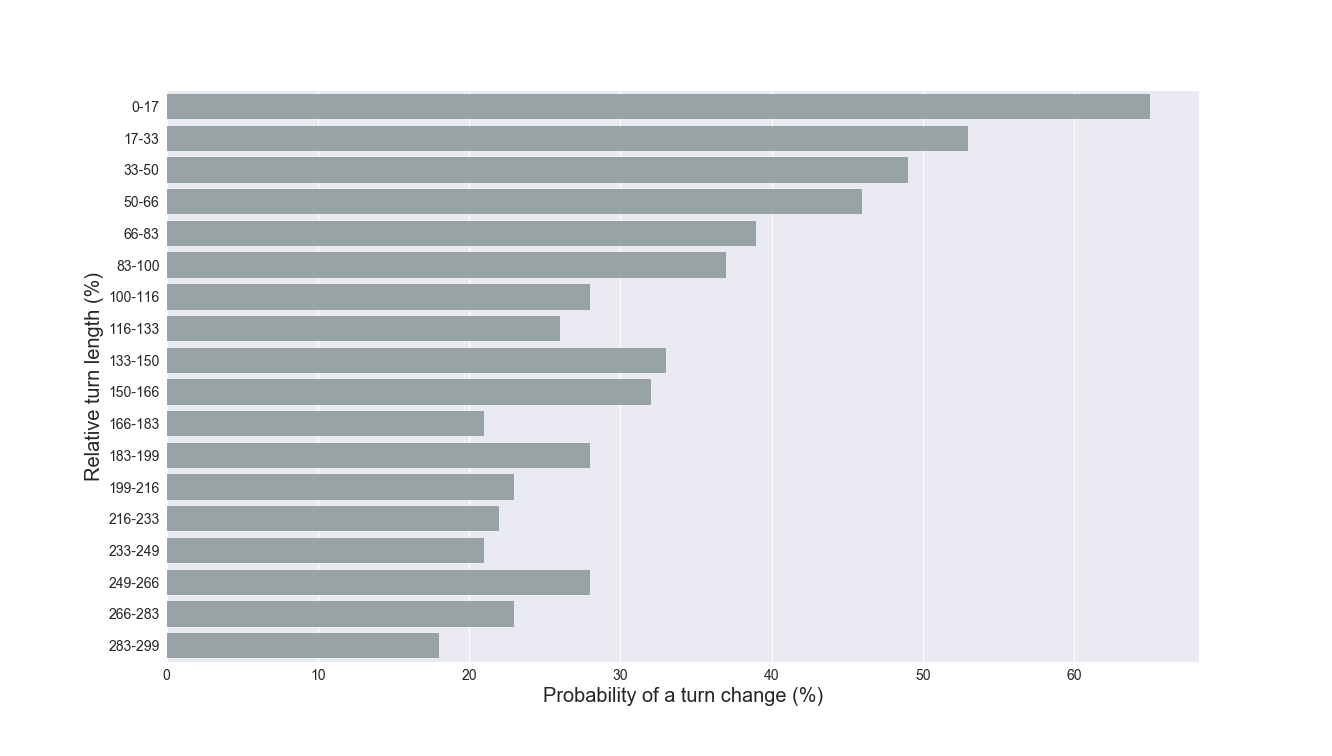
\includegraphics[width=\textwidth]{../scikitlearn/figures/f5.png}\vspace{-1em}
\caption{Relative turn length effect on probability of a turn change}
\label{fig:rtl:turn}
\end{figure}

The above finding is actually is opposite of our hypothesis that we stated in the introduction, in which we assumed that if a speaker's turn so far is less than her/her average then he/she would tend to keep speaking, and vice verse, if the speaker passed his/her average turn length he/she would tend to give up the turn. However, based on \ref {fig:rtl:turn}, we see the exact opposite.   We will explore this difference further in Section \ref{sec:opposite}.  None-the-less, we do see that this feature carries information, which can be used by machine learning, even though it is opposite of what we expected.


Next we measure the relation between values of relative floor control and probability of turn change.
As with relative turn length, we only include dialog acts after 120s into the conversation. We also divide the range of relative floor control into buckets such that each bucket contains roughly the same number of dialogs acts. We then count the number of dialog acts (regardless of the type) that led to a turn change and the total dialog acts for each bucket. Last, we compute the probability of a turn change by dividing the former by the latter.
The result is shown in Figure \ref {fig:rfc:turn}.  As we hypothesized in the introduction, we observe that high values of floor control correlate with the willingness of the current speaker to give up the turn. When the speaker has relative floor control scores above 50\% the speaker tends to keep the floor and avoid a turn change.
%
\begin{figure}[ht!]
\centering
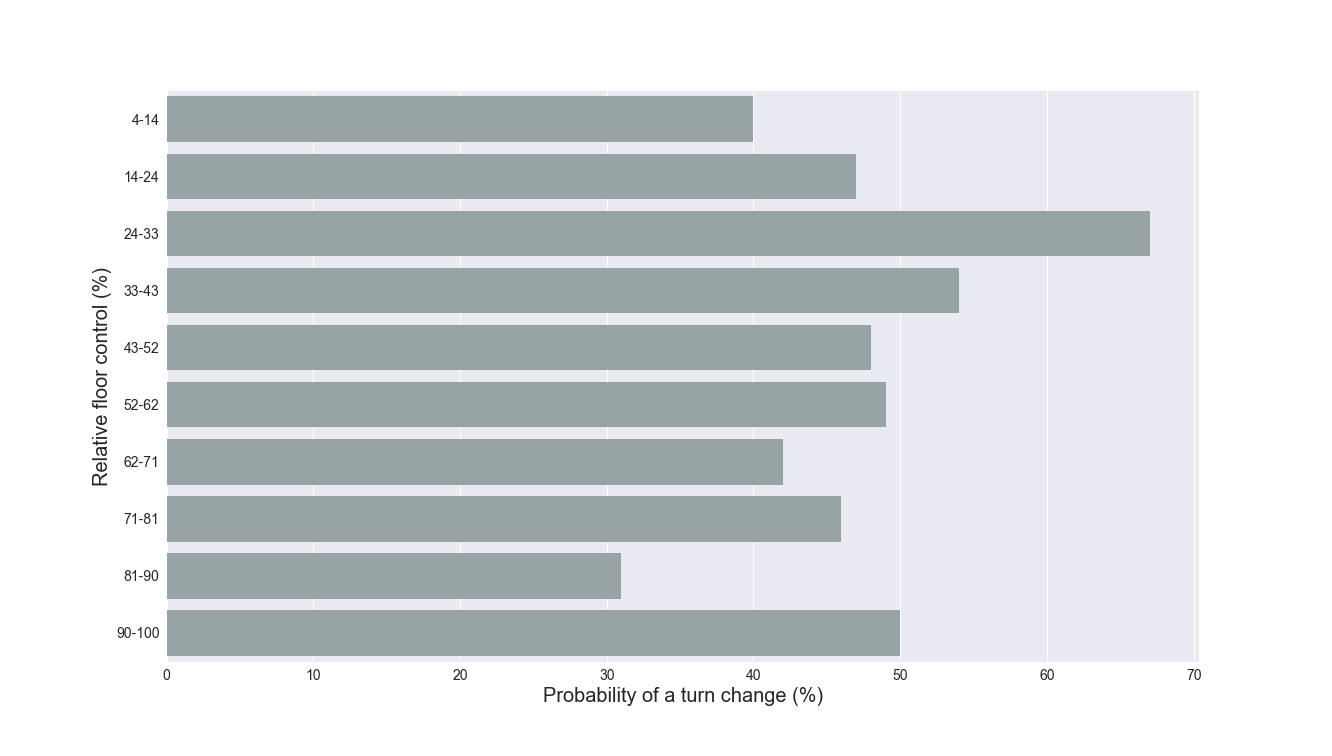
\includegraphics[width=\textwidth]{../scikitlearn/figures/f6.png}\vspace{-1em}
\caption{Relative floor control probability of turn change}
\label{fig:rfc:turn}
\end{figure}



\subsection{Influence of Dialogue Acts Types}

Next we explore the influence of dialog acts types (which are the local features in the theoretical model) on turn changes.
First we compute the distribution of dialog acts type over all the dialog acts in corpus.
Figure \ref{fig:act} plots the distribution of each dialog act in the corpus. Each bar is a count of the dialog act type, divided by the total number of dialog acts.  We observe that the majority of dialog acts are statements, backchannels and opinions. This might be due to the nature of the switchboard corpus, which consists mainly of casual conversations.
%
\begin{figure}[ht!]
 \centering
 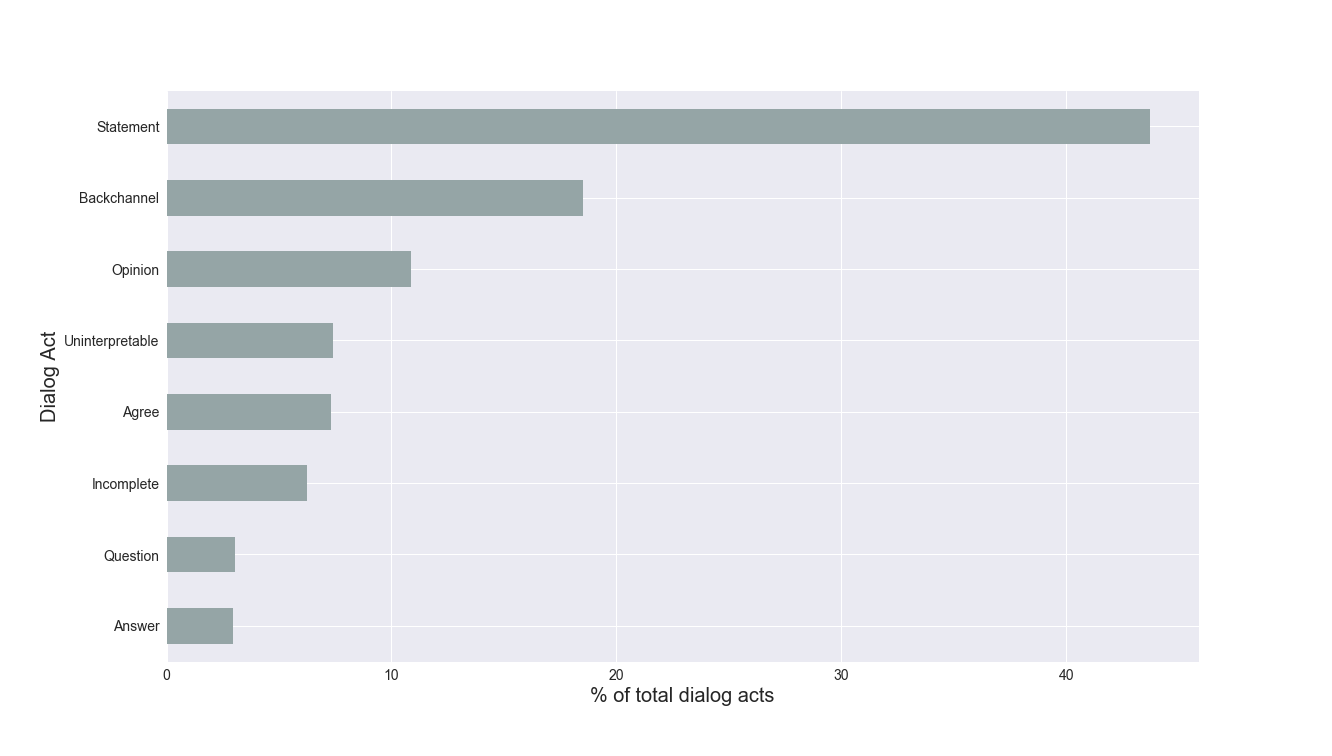
\includegraphics[width=\textwidth]{../scikitlearn/figures/f1.png}\vspace{-1em}
 \caption{Dialog act relative count}
 \label{fig:act}
 \end{figure}

Next we measure the correlation between dialog act type and the probability of a turn change.  In Figure \ref{fig:act:turnchange}, each bar measures the number of times a turn change occurred after a dialog act type divided by the total number of dialog acts of this type: the probability that a dialog act of the said type will lead to a turn change. We observe that the majority of back channels and questions (which are usually the first utterance in an question-answer adjacency pair) will lead to a turn change.
%
\begin{figure}[ht!]
\centering
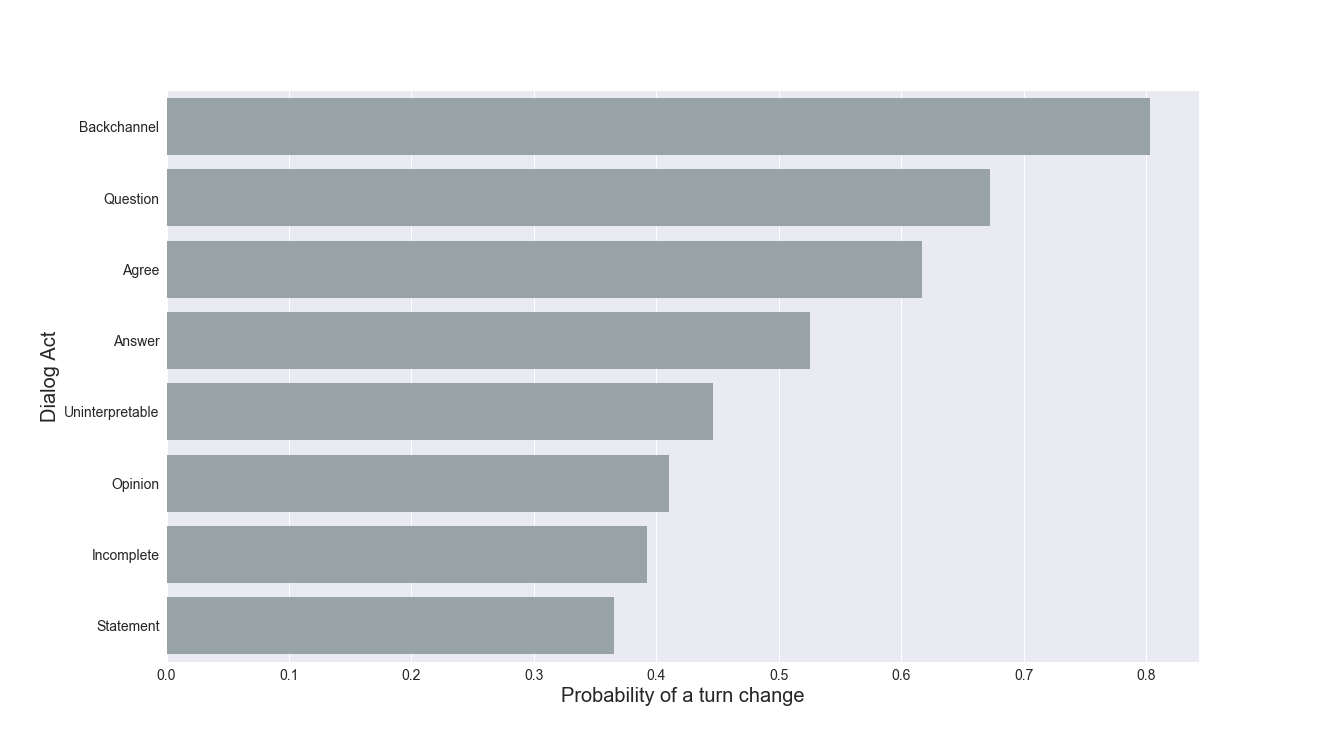
\includegraphics[width=\textwidth]{../scikitlearn/figures/f2.png}\vspace{-1em}
\caption{Dialog act probability of turn change}
\label{fig:act:turnchange}
\end{figure}

\subsection{Dialogue Act Types and Summary Features}

In this section we explore how the summary features are distributed for each dialog act. Moreover, we look at the score distribution for dialog acts that are followed by a turn change and ones that do not. In Figure \ref{fig:act:turn:rtl}, we see that, for most dialog act types,
the median relative turn length that led to a turn change is smaller than when it does not.  This suggests that speakers who are using the floor more than their
average turn length will tend to hold the floor even longer. This is consistent with our finding from Section \label{sec:data:summary}
that longer relative turn lengths result in a lower rate of turn-changes, but shows that it holds across speech act types as well.
%
\begin{figure}[ht!]
\centering
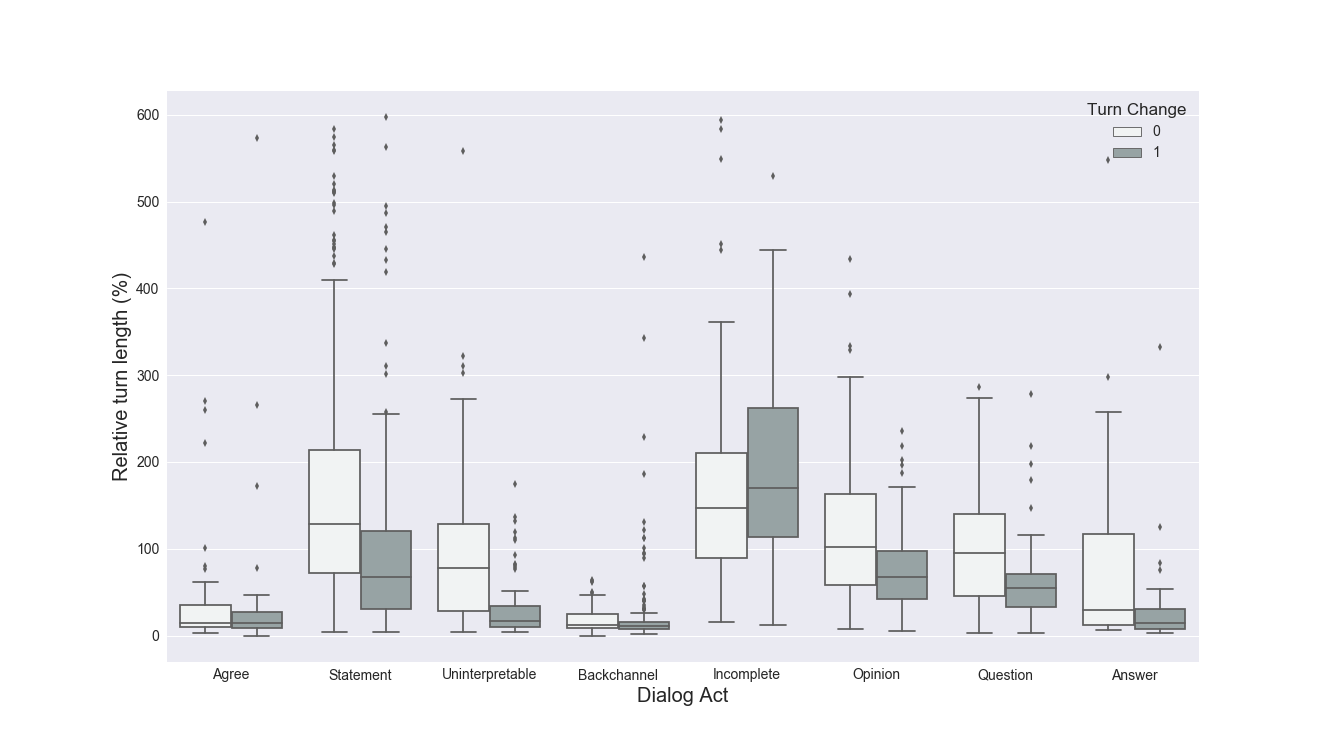
\includegraphics[width=\textwidth]{../scikitlearn/figures/f3.png}\vspace{-1em}
\caption{Relative turn length for dialog act type}
\label{fig:act:turn:rtl}
\end{figure}

Next we measure the relative floor control score for each type of dialog act.
In Figure \ref{fig:act:turn:rfc}, for each dialog act we show the distribution of relative floor control for acts that lead to turn changes and acts that do not. We see that for most of the dialog acts, the median score is about equal and close to 50\%.
%
We also observe that the median for relative floor control is slightly higher for each dialogue act when it not followed by a turn change, than when it is.  Again, this is consistent with our earlier result that higher values for relative floor control tend to lead to less turn-changes, but here we see that it also applies to each dialog act.
%
\begin{figure}[ht!]
\centering
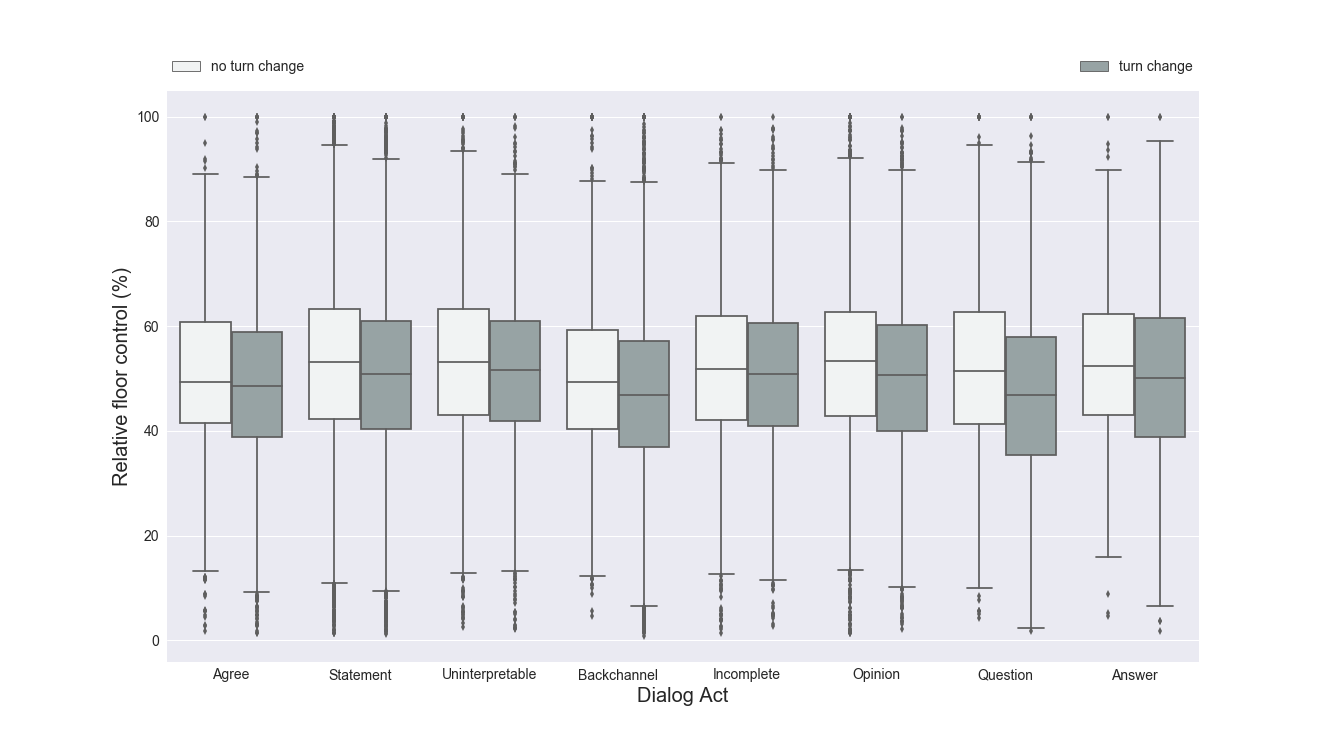
\includegraphics[width=\textwidth]{../scikitlearn/figures/f4.png}\vspace{-1em}
\caption{Relative floor control by dialog act}
\label{fig:act:turn:rfc}
\end{figure}

